\documentclass[a4paper,12pt]{report}
%\setlength{\columnsep}{0.7cm} % space between columns
\usepackage{filecontents}
\usepackage{gensymb}


\usepackage{lipsum}
\usepackage{fancyhdr}
\usepackage{titlesec}
\usepackage[spanish,es-tabla]{babel}
\usepackage[utf8]{inputenc}
\usepackage{amsmath,amssymb,amsthm}
\usepackage{afterpage}
\usepackage[left=2.5cm,right=2.5cm,top=2.5cm,bottom=2.5cm]{geometry}
\usepackage{tocloft}
\usepackage{enumerate} 
\usepackage{tikz}
\usetikzlibrary{shapes,arrows}

\usepackage{wrapfig}
\usepackage{graphicx,tabularx}
\usepackage{eurosym}
\usepackage{multicol}
\usepackage{multirow}
\usepackage{rotating}
%\usepackage{pdfpages}
\usepackage{pdflscape}
\usepackage{booktabs}
\usepackage[hyphens]{url}
\usepackage[document]{ragged2e}
\usepackage{subcaption}

\usepackage{tikz}
\usepackage[cuteinductors,americanvoltages,americancurrents,american]{circuitikz}

\newcommand{\newItemUrl}[1]{\href{#1}{#1}}
\newcommand{\tabitem}{~~\llap{--}~~}
\newcommand{\newItem}[1]{\multicolumn{3}{|p{11cm}|}{\tabitem #1}\\}

\newcommand\Tstrut{\rule{0pt}{2.6ex}} 
\newcommand\Zstrut{\rule{0pt}{3.2ex}} 
\newcommand\Bstrut{\rule[-0.9ex]{0pt}{0pt}}
\newcommand{\HRule}{\rule{\textwidth}{0.1mm}} 		
\usepackage{hyperref}
					% horizontal line and its thickness


\titleformat
{\chapter} % command
[hang] % shape
{  \normalfont\bfseries\Huge} % format
{} % label
{0.5ex} % sep
{
%	\centering 
} % before-code
[] % after-code


%nuevo comando

\newcommand{\tb}[1]{\textcolor{blue}{#1}}
\usepackage[english]{cleveref} %con este paquete si usas \cref{label} te pone automáticamente figura,ecuacion..

\newcommand{\refAnexo}[1]{(Anexo \ref{#1})}
\newcommand{\refFigura}[1]{(Figura \ref{#1})}
\newcommand{\refApartado}[1]{(Apartado \ref{#1})}

\title{\textbf{Control de drones mediante Reinforcement Learning en plataformas reales}}
\author{Miguel Fernández Cortizas}
\date{}

\newcommand{\grad}{$^{\circ}$}


\usepackage{dtk-logos} % for BibTeX stylized logo
\begin{document}
	
	\maketitle
	\tableofcontents
	\justify
	
	\chapter*{Resumen ejecutivo}
\section*{Introducción}
Los cuadrirrotores son vehículos aéreos no tripulados (\textit{UAV}) que se emplean para una gran variedad de tareas, por ejemplo, para la inspección de las palas de un aerogenerador en movimiento, el rodaje de una escena de acción en medio del mar o para facilitar la búsqueda de personas a las fuerzas del estado en labores de búsqueda y rescate. Estas aeronaves son iherentemente inestables, por lo que es necesario que cuenten con un sistema, que se encargue de mantener a la aeronave estable y facilitar su pilotaje. El desarrollo de los algoritmos de control que se ejecutan en estos sistemas, es un campo de interés debido a la utilización masiva de estas aeronaves, en tareas de naturalez muy diversa.

\newpage
	\chapter{Introducción}

Un multirrotor es un vehículo aeŕeo no tripulado o UAV (por sus siglas en inglés \textit{Unmanned Aerial Vehicles}) cuyos motores y hélices están orientadas de forma vertical. 

Estas aeronaves son mucho más maniobrables que una aeronave de ala fija, ya que, al poder mantenerse estables en una posición fija pueden realizar trayectorias de forma más precisa en espacios reducidos. Comparado con un helicóptero, el cual también puede mantenerse estable en un punto fijo, los multirrotores cuentan con un mantenimiento mucho más sencillo debido a la ausencia de complejos mecanismos.

Generalmente los motores de estas aeronaves son eléctricos, ya que poseen una gran velocidad de reacción y son capaces de manejar una gran cantidad de energía con rendimientos muy elevados. La energía que requieren se proporciona a través de baterías, lo cual limita el tiempo de vuelo de estas aeronaves, cuya autonomía es significativamente inferior a la de las aeronaves de ala fija o a la de los helicópteros con motores de combustión.

Todo esto, unido a su reducido precio, ha permitido que se potencie el uso masivo de este tipo de aeronaves para labores de: agricultura de precisión, topografía, inspección industrial y rodajes cinematográficos, entre otros usos.

Existen diversas topologías asociados a los multirrotores, dependiendo del número de motores y la disposición de éstos. En este trabajo vamos a trabajar con un cuadricóptero o cuadrirrotor (cuenta con cuatro motores) con disposición en X (\cref{Drone_en_X}).

\begin{figure}[htb!]
		\centering
		\includegraphics[width=0.3\textwidth]{introduccion/cuadrirrotorX.jpeg}
		\caption{Esquema cuadrirrotor en X}
		\label{Drone_en_X}
	\end{figure}

Se ha escogido esta topología de multirrotor debido a que posee el mínimo numero de motores que permiten un modelo sencillo de la dinámica de la aeronave.

\section{Motivación}

La popularidad de estas aeronaves en ámbitos como la inspección, la topografía o el ámbito cinematográfico requieren que la nave sea muy estable y que se pueda manejar con precisión. 
Todas estas aeronaves cuentan con un sistema electrónico que se encarga de que la nave sea estable y que facilite el pilotaje de la misma. A este sistema se le conoce como la controladora de vuelo o autopiloto.

\begin{figure}[htb!]
	\centering
	\includegraphics[width=0.3\textwidth]{introduccion/pixhawk4.jpg}
	\caption{Autopiloto comercial Pixhawk 4}
	\label{pixhawk}
\end{figure}

Actualmente, los autopilotos emplean algoritmos de control clásicos, basados la gran mayoría en reguladores PID para asegurar la estabilidad de la aeronave y permitir que se pilote de forma precisa. Debido a la peligrosidad de los drones (hélices afiladas girando a miles de revoluciones por minuto) no se pueden probar nuevos algoritmos de control sin tener sujeto al cuadricóptero.

Las teoría clásica de control empleada para estabilizar un cuadrirrotor requiere de un fino ajuste de los parámetros del modelo. Los últimos avances en aprendizaje automático han permitido que se desarrollen nuevos algoritmos de control empleando técnicas de aprendizaje por refuerzo y redes neuronales.



\section{Solución propuesta}

Con el objetivo de poder desarrollar nuevos algoritmos para el control de cuadrirrotores se ha desarrollado una plataforma, tanto hardware como software, que permita diseñar y probar estos algoritmos de forma segura. Esta plataforma esta constituida de :

\begin{itemize}
	\item \textbf{Entorno de simulación}, sobre el que se puedan probar los algoritmos de control en una aeronave simulada.
	\item \textbf{Cuadrirrotor con autopiloto de diseño propio}, será la aeronave donde se probarán los algoritmos diseñados. Al contar con una controladora de vuelo de diseño propio se pueden implementar los distintos algoritmos de control a bordo.
	\item \textbf{Interfaz con el autopiloto}, el cual comunica a la aeronave con un ordenador, el cual puede enviar comandos a la aeronave y recibir el estado de la misma. Esto permite la implementación de algoritmos \textit{en tierra}, en los cuales la computación del algoritmo se realiza en un ordendador en vez de en el microcontrolador del autopiloto. 
	\item \textbf{Banco de pruebas}, con distintas configuraciones en función del experimento que se desee realizar. Este banco permitirá probar los algoritmos de control de forma segura.
	
\end{itemize}


 Adicionalmente, se ha probado el rendimiento de distintos algoritmos de control basados en técnicas de aprendizaje por refuerzo para poder compararlos con los algoritmos de control clásicos PID.
 
 \section{Objetivos}
 Para poder llevar a cabo esta plataforma y poder implementar algún algoritmo basado en aprendizaje por refuerzo es necesario desgranar los objetivos principales en tareas de alcance más reducido:
 
 \begin{itemize}
 	\item \textbf{Entorno de simulación:}
 	\begin{itemize}
 		\item Estudio del estado del arte acerca de entornos de simulación para el diseño de algoritmos de control para cuadricópteros.
 		\item Estudio del estado del arte acerca de las técnicas de aprendizaje por refuerzo y el control de drones.
 		\item Adaptación del entorno de simulación a la plataforma escogida e integración con ROS.
 		\item Implementación de algoritmos clásicos en el entorno de simulación.
 		\item Diseño de nuevos algoritmos de control basados en aprendizaje por refuerzo y entrenamiento de los mismos.
 		\item Comparativa de los algoritmos en simulación.
 	\end{itemize}
 	\item \textbf{Cuadrirrotor con autopiloto de diseño propio:}
 	\begin{itemize}
 		\item Estudio del estado del arte acerca de los autopilotos comerciales.
 		\item Diseño y construcción completa del autopiloto: componentes, placa de circuito impreso y soldadura de componentes.
 		\item Programación del \textit{firmware} del autopiloto.
 		\item Diseño CAD de los componentes mecánicos del cuadrirrotor e impresion 3D de los mismos.
 		\item Montaje y esamblaje de todos los componentes de la aeronave.  
 	\end{itemize}
 	\item \textbf{Interfaz con el autopiloto:}
 	\begin{itemize}
		\item Diseño del protocolo de comunicación WiFi
		\item Integración del protocolo con ROS y con el autopiloto.
	\end{itemize}
	\item \textbf{Banco de pruebas}:
		\begin{itemize}
			\item Diseño CAD de las piezas de los distintos bancos de pruebas e impresión 3D de las mismas. 
		\end{itemize}
	\item \textbf{Experimentación de los algoritmos en el mundo real:} \tb{reducir o ampliar con los experimentos disponibles}
		\begin{itemize}
			\item Implementación a bordo de los algoritmos cĺásicos.
			\item Implementación externa de los algoritmos clásicos.
			\item Implementacion externa de los algoritmos basados en técnicas de aprendizaje por refuerzo. 
		\end{itemize}
 	

 \end{itemize}
	\chapter{\tb{Estado del arte}}

Las teoría clásica de control empleada para estabilizar un cuadricóptero requiere un fino ajuste de los parámetros del modelo. Los últimos avances en aprendizaje automático han permitido que se desarrollen nuevos algoritmos de control empleando técnicas de aprendizaje por refuerzo y redes neuronales.

 En 2004, HJ Kim et al. \cite{kim2004autonomous} emplearon algoritmos de \textit{reinforcement learing} para estabilizar (\textit{hoover}) un helicóptero y conseguir realizar maniobras acrobáticas.En 2006 Andrew Y. et al \cite{ng2006autonomous} siguieron con esta investigación consiguiendo que el helicóptero se estabilizara al revés (\textit{inverted hoover}). En 2010 Travis Dierks et al. \cite{dierks2010output} desarrollaron un controlador no lineal, basado en redes neuronales, para estabilizar un cuadricóptero y seguir trayectorias.
 
 Unos años después, en 2017 Jemin Hwangbo et al. \cite{hwangbo2017control} desarrollaron un método para controlar un quadricóptero con una red neuronal usando técnicas de \textit{reinforcement learning}. En 2018 William Koch et al. \cite{koch2019reinforcement} desarrollaron un entorno de simulación, GYMFC, para el desarrollo de sistemas de control empleando RL.


	\chapter{Fundamentos teóricos}

%\section{Control clásico}


%Una vez conseguida una estimación del estado en el instante $t$ ,  $S_t$ se necesita emplear un algoritmo de control que genere	las acciones $A_t$ correspondientes para llegar al estado $S_{t'}$ deseado de forma óptima.

%\tb{BUCLE DE CONTROL}


%Existe una gran cantidad de controladores clásicos que se pueden emplear para generar estos comandos, por ejemplo: PID o LQR.
%En este trabajo se han explorado 2 controladores: el primero de ellos se trata de un controlador clásico PID y el segundo consiste en un controlador no lineal modelizado por una red neuronal.

\section{Controlador PID}




Un regulador PID es un controlador lineal realimentado. Matemáticamente se expresa como 
\begin{equation}
	u(t) = \overbrace{\raisebox{0ex}[2.2\height]{$K_p e(t)$}}^\text{P} +\overbrace{K_i \int_{0}^{t}e(\tau)d\tau}^\text{I} + \overbrace{ K_d \frac{de(t)}{dt}}^\text{D}\;
\end{equation}




donde $e(t)$ es la señal de control, $u(t)$ representa la salida del regulador y $K_p,K_i,K_d$ son parámetros ajustables de los cuales depende la dinámica y la estabilidad del sistema. Como se puede observar, el regulador consta de tres partes: la parte proporcional (P) tiene en cuenta el error actual, la parte integral (I) tiene en cuenta el histórico de los errores y la parte derivativa (D) tiene en cuenta la estimación del error futuro.
\section{Redes neuronales artificiales} 
 Una red neuronal artificial (ANN) esta compuesta por un conjunto de nodos o perceptrones interconectados entre sí. Estos perceptrones se agrupan en capas ``ocultas'', se les atribuye este nombre debido a que todos los nodos de una capa se interconectan con todos los nodos de la capa anterior, por lo que después del aprendizaje de la red no se sabe cuales son los perceptrones de la capa anterior que influyen en un nodo.
 
 
 
 \begin{figure}[htb!]
 	\centering
 	\begin{tikzpicture}[]
 	\def\nodedist{35pt}
 	\def\layerdist{80pt}
 	\def\pindist{20pt}
 	
 	\tikzstyle{every pin edge}=[signal]
 	\tikzstyle{annot} = [text width=4em, text centered]
 	
 	\foreach \y in {1,...,3}
 	\node[inputnode, pin={[pin edge={latex-}, pin distance=\pindist]left:Entrada \y: $x_\y$}] 
 	(I\y) at (0,-\y*\nodedist) {$a_\y^{[0]}$};  
 	
 	\foreach \y in {1,...,4}
 	\node[hiddennode] 
 	(H\y) at ($(\layerdist,-\y*\nodedist) +(0, 0.5*\nodedist)$) {$a_\y^{[1]}$};
 	
 	\foreach \y in {1,...,1}
 	\node[outputnode, pin={[pin edge={-latex}, pin distance=\pindist]right:\Large$\hat y$}]
 	(O\y) at ($(I2) + (2*\layerdist, 0)$) {$a_\y^{[2]}$};
 	
 	\foreach \dest in {1,...,4}
 	\foreach \source in {1,...,3}
 	\draw[signal] (I\source) -- (H\dest);
 	
 	\foreach \dest in {1,...,1}
 	\foreach \source in {1,...,4}
 	\draw[signal] (H\source) edge (O\dest);
 	
 	\node[annot, above=4pt of H1] (hl) {Capa oculta};
 	\node[annot] at (I1 |- hl) {Capa de entrada};
 	\node[annot] at (O1 |- hl) {Capa de salida};
 	\end{tikzpicture}
 	\caption{Esquema de una red neuronal artificial}
 \end{figure}
 

Cada perceptron es la unidad mínima de computación de una ANN, estas unidades se dividen en dos partes, una parte lineal y una parte de activación o no lineal. En la parte lineal o parte ``Z'' se computa una regresión lineal de las salidas de los nodos anteriores.
 \begin{align}
 	z^{[l]}_i &= \sum_{j=0}^{n^{[l-1]}} {w_{ij}\cdot a^{[l-1]}_j} + b_i  \qquad &i=0,..,n^{[l]} \\
 	a^{[l]}_i &= g\left(z^{[l]}_i\right) \qquad  &i=0,..,n^{[l]}
 \end{align}
 El superíndice $[l]$ hace referencia a la capa en la que se encuentra el elemento. Siendo $n^{[l]}$ el número de nodos de la capa $l$-ésima.
 
 
 A los coeficientes $w_{ij}$ se les denomina los pesos del perceptrón y $b_i$ es el término independiente de la regresión. 
 
 
 \begin{figure}[htb!]
 	
 	\centering
 	\begin{tikzpicture}[
 	% define styles    
 	init/.style={ 
 		draw, 
 		circle, 
 		inner sep=2pt,
 		font=\Huge,
 		join = by -latex
 	},
 	squa/.style={ 
 		font=\Large,
 		join = by -latex
 	}
 	]
 	% Top chain x1 to w1
 	\begin{scope}[start chain=1]
 	\node[on chain=1] at (0,1.5cm)  (x1) {$a_1^{[l-1]}$};
 	\node[on chain=1,,label=above:\parbox{1cm}{pesos},join=by o-latex] (w1) {$w_1$};
 	\end{scope}
 	% Middle chain x2 to output
 	\begin{scope}[start chain=2]
 	\node[on chain=2] (x2) {$a_2^{[l-1]}$};
 	\node[on chain=2,join=by o-latex] {$w_2$};
 	\node[on chain=2,init] (sigma) {$\displaystyle\Sigma$};
 	\node[on chain=2,squa,label=above:{\parbox{2cm}{\centering Regresión lineal}}]   {$z_i^{[l]}$};
 	\node[on chain=2,squa,label=above:{\parbox{2cm}{\centering Función de\\ activacion}}]   {$a_i^{[l]}= g(z_i^{[l]})$};
 	\node[on chain=2,squa,label=above:Salida,join=by -latex] {$y_{out}$};
 	\end{scope}
 	% Bottom chain x3 to w3
 	\begin{scope}[start chain=3]
 	\node[on chain=3] at (0,-1.5cm) 
 	(x3) {$a_3^{[l-1]}$};
 	\node[on chain=3,join=by o-latex]
 	(w3) {$w_3$};
 	\end{scope}
 	% Bias
 	\node[label=above:\parbox{2cm}{\centering \text{$\;$} \\ $b$}] at (sigma|-w1) (b) {};
 	% Arrows joining w1, w3 and b to sigma
 	\draw[-latex] (w1) -- (sigma);
 	\draw[-latex] (w3) -- (sigma);
 	\draw[o-latex] (b) -- (sigma);
 	% left hand side brace
 	\draw[decorate,decoration={brace,mirror}] (x1.north west) -- node[left=10pt] {Entrada} (x3.south west);
 	
 	\end{tikzpicture}
 	\caption{Esquema de un perceptrón}
 	\label{esquema_perceptron}
 	
 \end{figure}
 
 La función $g(z)$ es la función de activación del nodo. Estas funciones proporcionan no linealidad a la red neuronal, permitiendo a estas la capacidad de generar modelos con grandes no linealidades. Las funciones de activación más frecuentes en la literatura son:
 
 \begin{itemize}
 	\item Función sigmoide: 
 	\begin{equation}
 	\sigma(z) = \frac{1}{1+e^{-z}} \qquad\qquad \sigma(z):\mathbb{R} \rightarrow [0,1]
 	\end{equation}
	\begin{figure}[htb!]
		\centering
		\begin{tikzpicture}[]
		\begin{axis}[ 
		%title=$\tanh(x)$,
		axis x line=middle, xmin=-4, xmax=4, xtick={-3,...,3}, xlabel=$x$,
		axis y line=middle, ymin=-2, ymax=2, ytick={-1,...,1}, ylabel=$f(x)$,
		legend pos=north west,
		legend style={empty legend, draw=none},
		scale only axis=true,
		width=8cm, height=4cm,
		thick,
		samples=101] 
		\addplot[blue, very thick] {1/(1+exp(-x))};
		%\addlegendentry{$\tanh(x)$}
		\end{axis}
		\end{tikzpicture}
		\caption{Función sigmoide}
	\end{figure}

	\item Tangente hiperbólica: 
	\begin{equation}
	\tanh(z) = \frac{e^z-e^{-z}}{e^z+e^{-z}} \qquad\qquad \tanh(z):\mathbb{R} \rightarrow [-1,1]
	\end{equation}
	
	\begin{figure}[htb!]
		\centering
		\begin{tikzpicture}[]
		\begin{axis}[ 
		%title=$\tanh(x)$,
		axis x line=middle, xmin=-4, xmax=4, xtick={-3,...,3}, xlabel=$x$,
		axis y line=middle, ymin=-2, ymax=2, ytick={-1,...,1}, ylabel=$f(x)$,
		legend pos=north west,
		legend style={empty legend, draw=none},
		scale only axis=true,
		width=8cm, height=4cm,
		thick,
		samples=101] 
		\addplot[blue, very thick] {tanh(x))};
		%\addlegendentry{$\tanh(x)$}
		\end{axis}
		\end{tikzpicture}
		
		\caption{Función tangente hiperbólica}
	\end{figure}

	\item ReLu (del inglés \textit{Rectified Linear Unit}): 
	
	\begin{equation}
		g(z) = \text{max}(0,z) \qquad\qquad g(z):\mathbb{R} \rightarrow [0,+\infty]
	\end{equation}
\\
	\begin{figure}[htb!]
		\centering
		\begin{tikzpicture}[]
		\begin{axis}[ 
		%title=$\tanh(x)$,
		axis x line=middle, xmin=-4, xmax=4, xtick={-3,...,3}, xlabel=$x$,
		axis y line=middle, ymin=-2, ymax=2, ytick={-1,...,1}, ylabel=$f(x)$,
		legend pos=north west,
		legend style={empty legend, draw=none},
		scale only axis=true,
		width=8cm, height=4cm,
		thick,
		samples=101] 
		\addplot[blue, very thick] {(\x < 0) * (0) + (\x > 0) * (\x)};
		%\addlegendentry{$\tanh(x)$}
		\end{axis}
		\end{tikzpicture}
		\caption{Función ReLu}
	\end{figure}
	

\end{itemize} 
  
 Para conseguir que la red neuronal realice predicciones precisas es necesario ajustar los pesos de la red, a este proceso es al que se denomina entrenamiento o aprendizaje. En el paradigma del aprendizaje supervisado este entrenamiento se realiza sometiendo a la red a ejemplos cuya salida es conocida. El objetivo de la red es minimizar el error de la esperanza de la estimación con respecto a la salida real del ejemplo. Formalmente, se define una función de coste $\mathcal{J}$ la cúal se quiere minimizar. Por ejemplo, una función de coste típica para problemas de clasificación binaria es la \textit{binary cross-entropy}:
 
 \begin{align}
 \mathcal{L}(\hat{y},y)&=-\big(y\log\hat{y} + (1-y)\log(1-\hat{y})\big)\\ 
 \mathcal{J}(w,b)&=\frac{1}{m}\sum_{i=1}^{m}{\mathcal{L}\big(\hat{y}^{(i)},{y}^{(i)}\big)}
 \end{align}
 donde $\hat{y}$ denota la estimación de la salida realizada por parte de la red, $y$ la salida conocida y $m$ el número de ejemplos. 
 
 Para minimizar esta función de coste, que depende de los pesos de la red, existen distintos métodos, uno de los más usados es el método del descenso de gradiente. Este método emplea la ``propagación hacia atrás'' (del inglés \textit{back propagation}) de la red neuronal, esto consiste en obtener las derivadas parciales de la función de coste con respecto a los pesos de cada nodo y actualizar estos pesos en la dirección opuesta al máximo gradiente.
 
 \begin{align}
 	w:= w - \alpha\; &\frac{\partial\mathcal{J}(w,b)}{\partial w}\\
 	b:= b - \alpha\; &\frac{\partial\mathcal{J}(w,b)}{\partial b}
 \end{align}
 
 donde $\alpha$ denota la tasa de aprendizaje, es decir, lo rápido que varian estos pesos.

 



\section{Aprendizaje por refuerzo}

El aprendizaje por refuerzo o \textit{Reinforcement learning} \cite{sutton2018reinforcement} es un área del aprendizaje automático o \textit{Machine Learning} en el que un agente interactúa con un entorno buscando la mejor acción a realizar en función de su estado actual.

Se diferencia de otras técnicas de aprendizaje automático es su enfoque orientado a la interacción directa con el entorno, sin basarse en un modelo completo del entorno o en un conjunto de ejemplos supervisados.

\subsubsection{Elementos del aprendizaje por refuerzo}
Además del agente y el entorno se pueden identificar tres elementos principales más en un sistema de aprendizaje con refuerzo:

\begin{itemize}
	\item[$\bullet$] \textbf{Política} (Proveniente del termino anglosajón \textit{policy}, el cual es el término empleado en el estado del arte). Define el conjunto de acciones que debe realizar el agente para conseguir maximizar su recompensa en función su estado, el cuál es percibido a través del entorno. La \textit{policy} constituye el núcleo del agente y nos permite determinar su comportamiento. Estas políticas pueden ser estocásticas.
	
	\item[$\bullet$] \textbf{Recompensa}. 
	Define el objetivo del agente en un problema de aprendizaje por refuerzo. En cada salto de tiempo (\textit{step}) el agente recibe una recompensa por parte del entorno (un número). 
	
	\item[$\bullet$] \textbf{Función de valor}. Representa la máxima recompensa que puede esperar obtener un agente desde un estado concreto, es decir, tiene en cuenta la recompensa a largo plazo, no solo la inmediata. 
		
\end{itemize}
Algunos algoritmos de aprendizaje por refuerzo requieren de la definición de un \textbf{modelo del entorno}. Este modelo permite predecir el comportamiento que va a tener el entorno a lo largo del tiempo.

\subsubsection{Procesos de decisión de Markov}

El aprendizaje por refuerzo emplea el marco formal de los procesos de decisión de Markov (\textit{MDP}) en los cuales para definir la interacción entre en agente y el entorno en términos de estados, acciones y recompensas.

Un proceso de decisión de Markov está compuesto por la 4-tupla $(S,A,P_a,R_a)$ donde:

\begin{itemize}
	\item \textbf{S} representa el estado del agente.
	\item \textbf{A} es el conjunto de acciones que puede realizar el agente. $A_s$ denota las acciones que puede realizar el agente desde un estado $s$.
	\item \textbf{$\boldsymbol{P_a(s,s')}$} = $Pr\big(s_{t+1} = s' \;|\; s_t = s , a_t = a  \big)$. Partiendo de un estado $s$, $P_a$ representa la probabilidad de pasar al estado $s'$ tomando la acción $a$.
	\item \textbf{$\boldsymbol{R_a(s,s')}$} denota la recompensa inmediata que recibiría el agente al realizar la transicion de $s$ a $s'$ mediante la acción $a$.
\end{itemize}

Estos procesos cumplen la propiedad de Markov, es decir, que el pasado no influye en el agente, lo único relevante es el estado actual.

El problema principal de los MDP es encontrar la secuencia de acciones que debe realizar el agente para maximizar la recompensa a largo plazo, es decir, encontrar la política $\pi$ 
óptima, que permita maximizar la recompensa. Una vez encontrada la política $\pi$ óptima el problema se reduce a una cadena de Markov, dado que la acción $a$ a realizar en un estado $s$ viene completamente definida por el estado $s$ y la probabilidad $P_a$. 

La política $\pi$ óptima es aquella que maximize la recompensa acumulada, es decir, la suma decontada de las recompensas instantáneas percibidas por el entorno:

\begin{equation}
	\sum_{t_0}^{\infty}\gamma^t R_{a_t}(s_t,s_{t+1}) \qquad \text{las acciones $a_t$ vienen dadas por $\pi(s_t)$}
\end{equation}

donde $\gamma$ es el factor de descuento, el cual debe cumplir $0 \le \gamma \le 1$, cuanto mayor sea este factor menos importante es la recompensa inmediata. 

En los casos en los las probabilidades $P_a$ o las recompensas $R_a$ no se conocen a priori, es necesario emplear técnicas de aprendizaje por refuerzo para obtener esa política.

En estos problemas es util definir el Q-valor

\begin{equation}
Q(s,a) = \sum_{s'}P_a(s,s')\big(R_a(s,s')+\gamma V(s') \big)
\end{equation}

\subsection{DQN}
\subsection{DDPG}
\subsection{TRPO}
\subsection{PPO}
	\chapter{Metodología (\tb{Problem Formulation})}

Además del desarrollo de la plataforma de la aeronave, otro objetivo del trabajo es intentar estabilizar un UAV usando algoritmos de control basados algoritmos de aprendizaje automático. Los principales componentes que intervienen en el agente son el estado, las acciones y la recompensa, para cada problema hay un conjunto que estados, acciones y funciones de recompensa que pueden llevar a que el agente aprenda.

\section{Diseño del estado}
 El autopiloto cuenta con 2 IMUs para poder obtener datos sobre su estado. Se quiere estabilizar el dron en una orientación concreta, por lo tanto el estado que se ha diseñado consta de 6 parámetros:
\begin{equation}
	S=(\varphi,\theta,\psi,\dot\varphi,\dot\theta,\dot\psi) \qquad\qquad \varphi,\theta,\psi,\dot\varphi,\dot\theta,\dot\psi \in [-1,1]
\end{equation} 

Siendo $\varphi,\theta$ y $\psi$ los ángulos de alabeo (\textit{roll}), cabezeo (\textit{pitch}) y guiñada (\textit{yaw}) del dron  y $\dot\varphi,\dot\theta$ y $\dot\psi$ sus respectivas velocidades. Para favorecer la convergencia del aprendizaje, se ha normalizado el estado para que todas sus componentes estén comprendidas dentro del intervalo $[-1,1]$.

Los ángulos proporcionan información sobre el estado actual y la velocidad angular sobre los estados pasados y los posibles estados futuros, es decir, proporciona cierta información temporal. 

\section{Diseño de las acciones}
Al trabajar con un quadricóptero podemos actuar sobre la potencia que se le entrega a los motores, por lo que cada acción que realice el agente constará de 4 campos:
\begin{equation}
	A = (T_1,T_2,T_3,T_4) \qquad\qquad T_i \in [-1,1]
\end{equation}

Siendo $T_i$ la potencia \textit{(Thrust)} normalizada entregada a cada motor. Un valor de $T_1=-1$ significa que el motor 1 estaría girando a la mínima potencia permitida y un valor de $T_1=1$ corresponde a que el motor 1 estaría girando a la máxima potencia.\\

Las señales de control que admiten los variadores es una señal PWM de 50Hz cuyo ancho de pulso debe estar entre 1ms y 2ms. Un ancho de pulso de 1ms se corresponde con la mínima velocidad el motor y un ancho de 2ms con la máxima, veáse \cref{hardware_ESCWAVE}.\newpage

\begin{figure}[htb!]
	\centering
	\includegraphics[width=0.6\textwidth]{hardware/ESCWaves}
	\caption{Formas de onda que recibe un variador}
	\label{hardware_ESCWAVE}	
\end{figure}

 Para realizar esta transformación del dominio $[-1,1]$ al dominio [1000,2000] $\mu$s se han empleado la siguiente expresión

\begin{equation}
	P_i= T_i \cdot 1000 \cdot \alpha + \beta \qquad \qquad i=0,...,3
\end{equation}\\
siendo $P_i$ el ancho del pulso enviado al ESC, $\alpha \in [0,1]$  es el porcentaje de la potencia total que puede manejar el controlador y $\beta \in [0,2000]$ es la velocidad base que tienen los motores. Esta velocidad base permite que el dron pueda variar su altura y que se pueda autosustentar. 

\section{Diseño de la función de recompensa y ajuste de hiperparámetros}

La búsqueda de la función de recompensa y la elección de los hiperparámetros que aseguraban la convergencia de los distintos algoritmos, se ha realizado mediante un proceso cíclico, en el que, se realizaba una hipótesis sobre la posible forma de la función de recompensa o el posible valor de un hiperparámetro que podría mejorar el algoritmo. Posteriormente se ejecutaba el algoritmo y se comparaban los resultados de este entrenamiento con los resultados previos. Para disminuir el tiempo de los entrenamientos, se simplificaba el problema del control del cuadricóptero a un único eje de giro. Con esto se redujo el tiempo que se tardaba en completar el ciclo.

\tb{diagrama ciclo}


\subsubsection{Función de recompensa}
La función de recompensa rige la forma en la que la red va a configurar sus pesos, por lo tanto, cómo se va a comportar el agente en un estado determinado. Para conseguir que el agente responda de la forma deseada se han probado una gran variedad de funciones de \textit{reward}, optando finalmente por:
\begin{equation}
	%R_t = \left( 1-\frac{|\varphi - \varphi_{ref}| + |\theta-\theta_{ref}| + |\psi- \psi_{ref}|}{3}\right)^3
	R_t = \left( 1-\frac{|\varphi|  + |\theta| + |\psi|}{3}\right)^n
\end{equation}
Sea $\gamma= \frac{|\varphi|  + |\theta| + |\psi|}{3} $ entonces $R_t = (1- \gamma)^n$, con $n \in \mathbb{N}$. Aumentando el valor de $n$ podemos conseguir funciones de recompensa con pendientes más pronunciadas.

	\begin{figure}[htb!]
\centering
	
	\begin{subfigure}{0.32\textwidth}
		\centering
		\begin{tikzpicture}[]
		\begin{axis}[ 
		%title=$\tanh(x)$,
		domain=0:1, restrict y to domain=-10:10,
		axis x line=middle, xmin=0, xmax=1, xtick={0,0.5,...,1}, xlabel=$\gamma$,
		axis y line=middle, ymin=0, ymax=1, ytick={0,...,1}, ylabel=$r_t$,
		y label style={at={(current axis.below origin)},anchor=south east},
		scale only axis=true,
		width=0.7\textwidth, height=3.5cm,
		samples=40] 
		\addplot[blue, very thick] {(1-(\x))^4};		\end{axis}
		
		%\addlegendentry{$\tanh(x)$}	
		\end{tikzpicture}
	\end{subfigure}
\begin{subfigure}{0.32\textwidth}
	\centering
	\begin{tikzpicture}[]
	\begin{axis}[ 
	%title=$\tanh(x)$,
	domain=0:1, restrict y to domain=-10:10,
	axis x line=middle, xmin=0, xmax=1, xtick={0,0.5,...,1}, xlabel=$\gamma$,
	axis y line=middle, ymin=0, ymax=1, ytick={0,...,1}, ylabel=$r_t$,
	y label style={at={(current axis.below origin)},anchor=south east},
	scale only axis=true,
	width=0.7\textwidth, height=3.5cm,
	samples=40] 
	\addplot[blue, very thick] {(1-(\x))^4};
	\end{axis}
	
	%\addlegendentry{$\tanh(x)$}	
	\end{tikzpicture}
\end{subfigure}
\begin{subfigure}{0.32\textwidth}
	\centering
	\begin{tikzpicture}[]
	\begin{axis}[ 
	%title=$\tanh(x)$,
	domain=0:1, restrict y to domain=-10:10,
	axis x line=middle, xmin=0, xmax=1, xtick={0,0.5,...,1}, xlabel=$\gamma$,
	axis y line=middle, ymin=0, ymax=1, ytick={0,...,1}, ylabel=$r_t$,
	y label style={at={(current axis.below origin)},anchor=south east},
	scale only axis=true,
	width=0.7\textwidth, height=3.5cm,
	samples=40] 
	\addplot[blue, very thick] {(1-(\x))^10};
	\end{axis}
	
	%\addlegendentry{$\tanh(x)$}	
	\end{tikzpicture}
	
\end{subfigure}
	\caption{Funciones $R_t$ para distintos valores de $n = 2,4,10$ respectivamente}
\end{figure}

Esta función $R_t:[0,1]\rightarrow [0,1] \;\; \forall n \in \mathbb{N} > 0$ por lo que al proporcionar valores entre 0 y 1, favorece la velocidad del entrenamiento. Además toda la recompensa es positiva, por lo que el agente intentará mantenerse la mayor cantidad de tiempo posible sin reiniciar el episodio, esto es muy importante para conseguir la convergencia del entrenamiento en los escenarios en los que se desea que el cuadricoptero se encuentre siempre dentro de una región concreta del espacio. 

\subsubsection{Ajuste de hiperparámetros}

Debido a las diferentes naturalezas de cada uno de cada uno de los algoritmos que se han empleado: DDPG, TRPO y PPO , cada uno cuenta con un conjunto distinto de hiperparámetros que ajustar. La implementación de estos algoritmos que se ha empleado (\textit{stable-baselines}) contiene unos hiperparámetros por defecto, los cuales suelen hacer que los algoritmos converjan.

Por lo general, no ha sido necesario modificar mucho estos parámetros por defecto, a excepción del valor de la constante $\epsilon$ en el algoritmo PPO. Este parámetro modifica el tamaño de la región de confianza del algoritmo, acotando el tamaño de los pasos que se toman en el curso de cada actualización de la política. Se observó que el valor por defecto de este parámetro $\epsilon_{defecto} = 0.2$ era demasiado grande, por lo que la política divergía. A medida que este parámetro se disminuye, se aumenta la estabilidad del aprendizaje, sin embargo, también se ralentiza mucho. Es por esto que el valor de éste hiperpaŕametro se ha ido modificando a lo largo de los experimentos, para poder conseguir el entrenamiento más rápido, capaz de converger de forma estable. 




	\chapter{Hardware}
Un cuadricóptero o cuadrirrotor es una aeronave no tripulada (UAV) que está propulsada por cuatro motores cuyas hélices están orientadas verticalmente.Se ha diseñado y construido un cuadrirrotor casero para poder probar en la realidad el control del dron. 

Un cuadricóptero convencional cuenta con: un chasis o \textit{frame} que lo sustenta, cuatro motores y la electrónica necesaria para controlarlos, una controladora de vuelo que lo comanda y baterías que le proporcionan energía.

A continuación se detallará como són las distintas partes del dron que se ha fabricado.
\section{Cuadro}
El \textit{frame} está compuesto por perfiles de aluminio y piezas de PLA fabricadas mediante impresión 3D. Cuenta con un nivel para alojar los motores, la receptora de radio y la controladora de vuelo y otro nivel para la batería. Todas las piezas de PLA son de diseño propio y se han realizado mediante software CAD.\\


\tb{\tb{\huge imagenes modelo CAD}}.
\section{Motores y variadores(ESC)}
El dron cuenta con 4 motores sin escobillas (\textit{brushless}) LHI MT2204 II de 2300KV con una tensión de alimentación entre 7.2 V y 11.1 V (2s -3s en una batería LiPo) y una corriente continua máxima de 16A.


Estos motores son trifásicos, es decir, se alimentan con 3 corrientes alternas monofásicas de igual frecuencia y amplitud, desfasadas 120\grad \;eléctricos. Para obtener estás formas de ondas a partir de la corriente continua de las baterias, se utilizan los variadores o \textit{ESC}.\\


\newpage
\begin{figure}[htb!]
	\centering
	\begin{subfigure}{0.4\textwidth}
		\centering
		\includegraphics[width=0.8\textwidth,height=0.2\textheight]{hardware/motores.jpg}
		\caption{Motores LHI MT2204 II empleados}
		\label{hardware:motores}
	\end{subfigure}
	\begin{subfigure}{0.4\textwidth}
		\centering
		\includegraphics[width=0.8\textwidth,height=0.2\textheight]{hardware/esc.jpg}
		\caption{ESC Multistar Race 4 in 1 30A BLHeli empleado}
		\label{hardware:esc}
	\end{subfigure}
\end{figure}


Un variador o \textit{ESC (Electronic speed control)} es un circuito electrónico que controla y regula la velocidad de un motor eléctrico. \\

\tb{\Huge Profundicar en las ondas generada por el ESC}
\section{Baterias}
Para alimentar al dron, se han elegido baterias tipo LiPo por su alta tasa de descarga (la batería que se ha escogido es capaz de entregar hasta 130 A) y la su estabilidad en la tensión mientras están cargadas.


\begin{figure}[htb!]
		\centering
		\includegraphics[width=0.8\textwidth]{hardware/curvaLipo}
		\caption{Curva típica de descarga de una bateria LiPo (fuente: ProtoTalk.net)}
		\label{hardware:curvaLipo}

\end{figure}


\section{Autopiloto}

En los drones, el sistema que se encarga de estabilizar al cuadricóptero y hacerlo pilotable se denomina la controladora de vuelo o el Autopiloto. Existe una gran variedad de controladoras en el mercado, pero para este trabajo se ha diseñado una controladora propia con el fin de poder tener acceso a todos los sensores y a implementar el algoritmo de control de forma óptima. El autopiloto consta de 3 partes diferenciadas: la electrónica de potencia, el microcontrolador y los sensores. A continuación \tb{se tratará} sobre estas partes con más detalle.\\


\tb{Estaría bien un par de imágenes de la PCB (anverso y reverso)}\\

\begin{figure}[htb!]
	\centering
	\includegraphics[width=0.8\textwidth]{hardware/carl_board}
	\caption{Autopiloto CaRL (\textit{Cuadcopter with autopilot based on Reinforcement Learning}).}
	\label{hardware:carl_board}	
\end{figure}



\subsection{Fase de Potencia}

Con el fin de poder gestionar la potencia entregada por las baterias a la placa y a los motores se ha diseñado una etapa de potencia en la que se debe mencionar dos partes: el interruptor de potencia y el regulador a 3.3 Voltios.

\subsubsection{Interruptor de potencia}

Los motores del dron pueden llegar a consumir 12 Amperios cada uno, lo que los cuatro motores pueden llegar a consumir 48 Amperios. Un interruptor con tamaño reducido no puede manejar tanta corriente, por ello se ha empleado un transistor MOSFET de canal P por el que pueden circular hasta 100 Amperios, con el fin de abrir o cerrar el paso de corriente desde las baterías al resto de la placa. El MOSFET se controla con un interruptor de poca potencia entre drenador y puerta.\\

Cuando se cierra el interruptor se alimenta directamente al ESC y al regulador de tensión.


\subsubsection{Regulador a 3.3V}

La eléctronica digital de la PCB se alimenta y emplea lógica a 3.3 Voltios, por lo que no la podemos conectar a las baterías de 11.1 Voltios.  Para adecuar la tensión se ha escogido un regulador Step-down de tipo Buck (Figura \ref{hardware:Buck}) \tb{(¿explico como funciona un convertidor Buck?)}. El circuito integrado que se encarga de conmutar la fuente es el chip AP3211.
\begin{figure}[htb!]
	\centering
		\begin{circuitikz}[american voltages,european resistors,scale=1]	
		
		\draw
		(0,2) to [V=$V_{in}$]  (0,-2)
		(0,2) to ++(1.5,0)
		++(0.5,0)node[nigfete,bodydiode,rotate=90]{}  to ++(2,0);
		
		\draw 
		(0,-2) to ++(4,0)
		++(0,0)[sD*] to ++(0,4)
		;
		\draw 
		(4,2) to [L=$L$,i=$i_L$] ++(3,0);
		\draw
		(7,2) to [C,l_=$C$] ++(0,-4)
		;
		
		\draw
		(7,2) to ++(3,0) 
		to [R =$R_{load}$,i=$i_{Load}$] ++(0,-4)
		to (0,-2)
		;
		\draw (2,0.75)node[]{\footnotesize SW};
		\draw (9.5,0.5)[short] to ++ (0,-0.5);
		\draw[-latex]
		(9.5,0)node[left] {$V_{out}$} to ++(0,-0.5);	
		
	\end{circuitikz}
	\caption{Esquema de un convertidor Buck}
	\label{hardware:Buck}
\end{figure}


\subsection{El microcontrolador (ESP32)}

El microcontrolador por el que se ha optado para este Autopiloto es el ESP32, un microcontrolador de doble núcleo con dos CPUs XTensaL6 con arquitectura Harvard \cite{ESP32TechnicalReference}. El ESP32 tiene una frecuencia de reloj de hasta 240MHz ,y cuenta con una antena WiFi a 2,4 GHz y conexión Bluetooth 4.2 BLE \cite{ESP32DataSheet}. Los motivos por los que se ha decidido emplear este microcontrolador son:
\begin{itemize}
	\item Elevada frecuencia de procesamiento y dos nucleos de procesamiento.
	\item Antena WiFi incorporada.
	\item Bajo consumo de potencia.
\end{itemize}

\par Para poder programar el microcontrolador se utiliza un convertidor USB (Bus Serie Universal) a UART (Transmisor-Receptor Asíncrono Universal) que permite conectar por USB el microcontrolador para poder programarlo y hacer depuración utilizando comunicaciones Serial. El chip que realiza esta funcion es el CP2104.

\subsection{Sensores}
La principal fuente de información procedente del exterior que recibe una controladora de vuelo se la proporcionan las unidades de medición inercial (IMU). Las IMUs son dispositivos electrónicos que son capaces de medir aceleraciones, velocidades y detectar la orientación de un sistema. El principal problema de estos sensores es que suelen sufrir error acumulativo.
\tb{¿profundizo en los sensores MEMS (imus electrónicas )?}\\


\par Otros sensores utilizados frecuentemente en los autopilotos son brújulas (se encuentran integrados en la IMU para corregir errores de orientación) y barómetros (para estimar la altitud a la que se encuentra el dron).\\
\medskip

Nuestro autopiloto cuenta con dos IMUs de 9 Grados de Libertad y un barómetro para conseguir una mejor estimación del estado del cuadricóptero:

\begin{enumerate}
	\item \textbf{BNO 055 (BOSCH)}: El circuito integrado de Bosch es un sensor "inteligente" que incluye los sensores y la fusión de las lecturas de los distintos sensores en un único componente.
	Este sensor nos proporciona estimaciones del estado con muy poca deriva. \tb {argumentar un poco mejor}
	
	\item \textbf{MPU 9250 (TDK InvenSense)}: El sensor inercial de TDK tiene una mejor respuesta dinámica, aunque la fusión de las lecturas del sensor se realiza externamente en el microcontrolador del dron.
	
	\item \textbf{BMP388 (BOSCH)}:
\end{enumerate}

%\section{Otros (Receptora radio)}

\section{Banco de pruebas}
Para poder realizar la experimentación real de forma segura, se ha diseñado una base para sujetar al drone permitiendo que rote en roll pitch y yaw de forma restringida.

La estructura de sujección esta formado por 2 juntas esféricas acopladas una a continuación de la otra, para permitir la rotación en el espacio. 
\\

\tb{\huge imagen rotulas y/o CAD }
\\

Los límites físicos de las rótulas permiten que el dron tome orientaciones comprendidas entre:
\begin{align*}
	 -60 \degree &\le \varphi \le 60\degree \quad \;\;\;  \text{Roll}\\ 
	 -60 \degree&\le \theta \le 60\degree \qquad  \text{Pitch} \\
	 -180 \degree&\le \psi \le 180\degree\quad \;  \text{Yaw}
\end{align*}


	\chapter{Experimentos}
Debido a que el trabajo tiene dos partes principales claramente diferenciadas, se han diseñado distintos tipos de experimentos para la evaluación de cada parte:un conjunto de experimentos en simulación para probar el rendimiento de los algoritmos de aprendizaje por refuerzo y un conjunto experimentos en real para probar la plataforma hardware y el diseño del autopiloto.
\section{Experimentos en simulación}
Con el ánimo de probar los distintos algoritmos de control basados en aprendizaje por refuerzo, se han diseñado diversos experimentos para comparar el rendimiento de estos algoritmos con el de un PID clásico. 
\subsubsection{Control en 1 GdL (\textit{Roll})}


\begin{figure}[htb!]
	\centering
	\includegraphics[width=\textwidth]{experimentos/sim_onlyroll}
	\caption{Estabilización en \textit{roll} en un entorno simulado.}
	\label{mat_lab_graph}	
\end{figure}

\subsubsection{Control en 1 GdL (\textit{Pitch})}
\begin{figure}[htb!]
	\centering
	\includegraphics[width=\textwidth]{experimentos/sim_onlypitch}
	\caption{Estabilización en \textit{pitch} en un entorno simulado.}
	\label{mat_lab_graph}	
\end{figure}

\subsubsection{Control en los 3 GdL}


\begin{figure}[htb!]
	\centering
	\includegraphics[width=0.9\textheight,angle=90]{experimentos/3_angles_real}
	\vspace{0.5cm}
	\caption{Estabilización en \textit{roll}, \textit{pitch y \textit{yaw}} simultáneamente}
	\label{tl_pr}	
\end{figure}

\section{Experimentos en real}
Para la evaluación de la plataforma de vuelo , el diseño del cuadricóptero y del autopiloto, se han realizado distintos experimentos para intentar controlar la aeronave con algoritmos PID en cascada a una frecuencia de 70Hz.
\subsubsection{Control en 1 GdL (\textit{Pitch})}

En este experimento se ha empleado la rótula de 1 GdL que únicamente permite el movimiento en \textit{pitch}.

\begin{figure}[htb!]
	\centering
	\includegraphics[width=\textwidth]{experimentos/real_only_pitch}
	\caption{Estabilización en \textit{pitch}. Las flechas marcan los tiempos en los que se perturbó al sistema.}
	\label{mat_lab_graph}	
\end{figure}

Se observa que el sistema es capaz de estabilizarse y que reacciona ante las perturbaciones externas de forma ágil. Por otro lado, también podemos observar ruido en la zona estable, además de poseer un pequeño error de posición de unos 2\grad.

\begin{figure}[htb!]
	\centering
	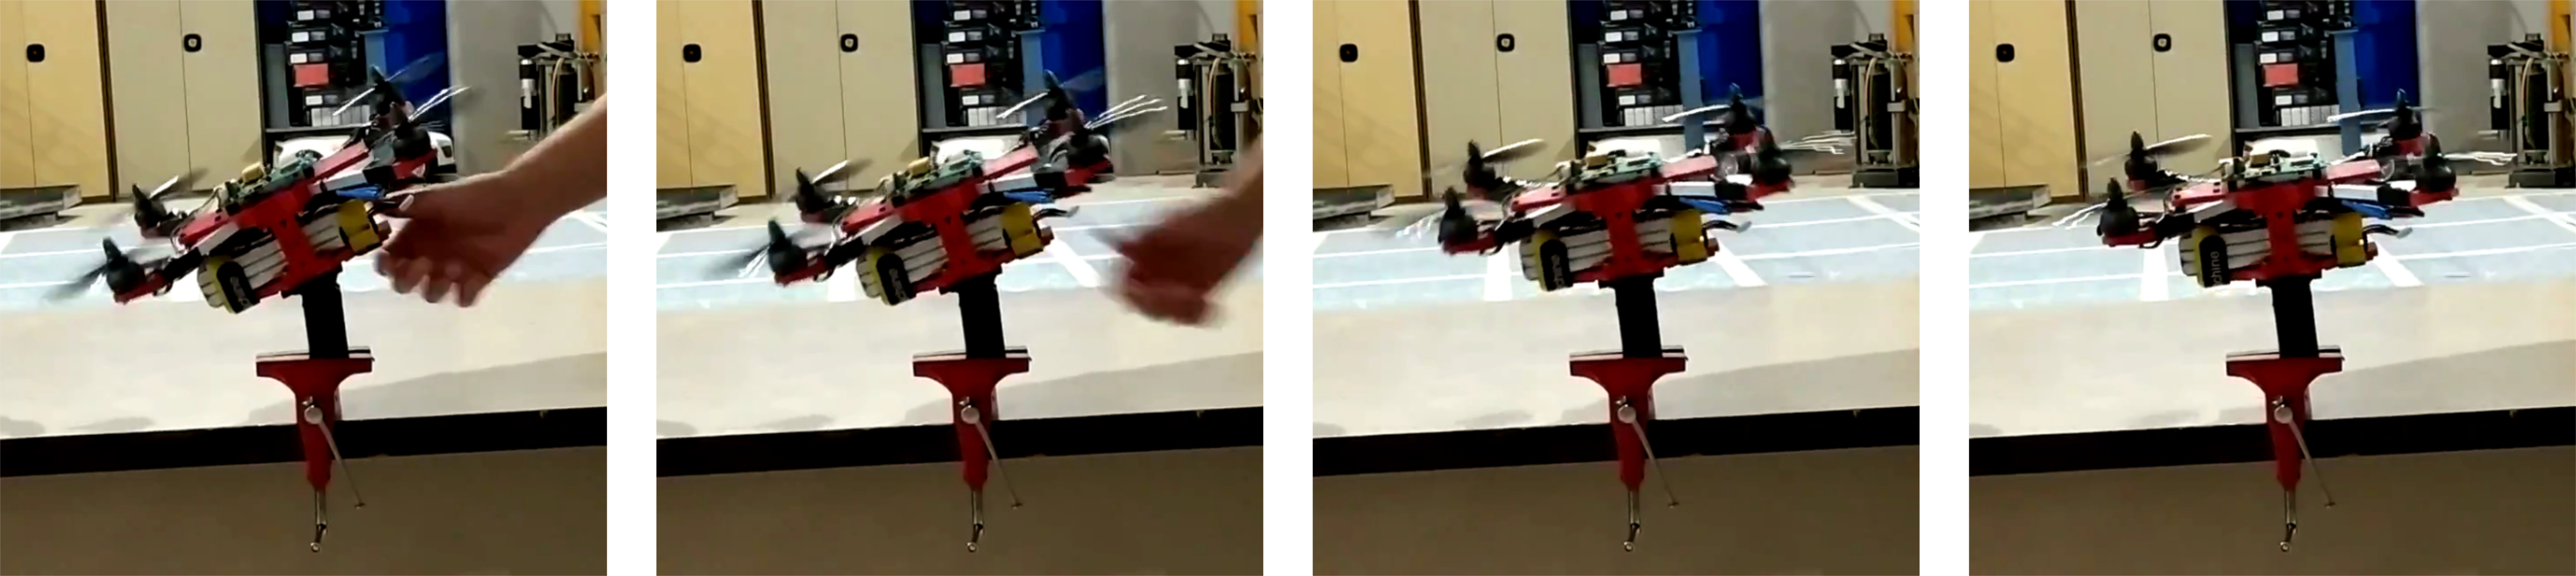
\includegraphics[width=\textwidth]{experimentos/time_lapse_pitch_real}
	\caption{Estabilización en \textit{pitch}}
	\label{tl_pr}	
\end{figure}


\subsubsection{Control en 1 Gdl (\textit{Roll})}
En este experimento se ha empleado la rótula de 1 GdL que únicamente permite el movimiento en \textit{roll}.

\begin{figure}[htb!]
	\centering
	\includegraphics[height=0.18\textheight,width=\textwidth]{experimentos/real_only_roll}
	\caption{Estabilización en \textit{roll}. Las flechas marcan los tiempos en los que se perturbó al sistema.}
	\label{mat_lab_graph}	
\end{figure}

\begin{figure}[htb!]
	\centering
	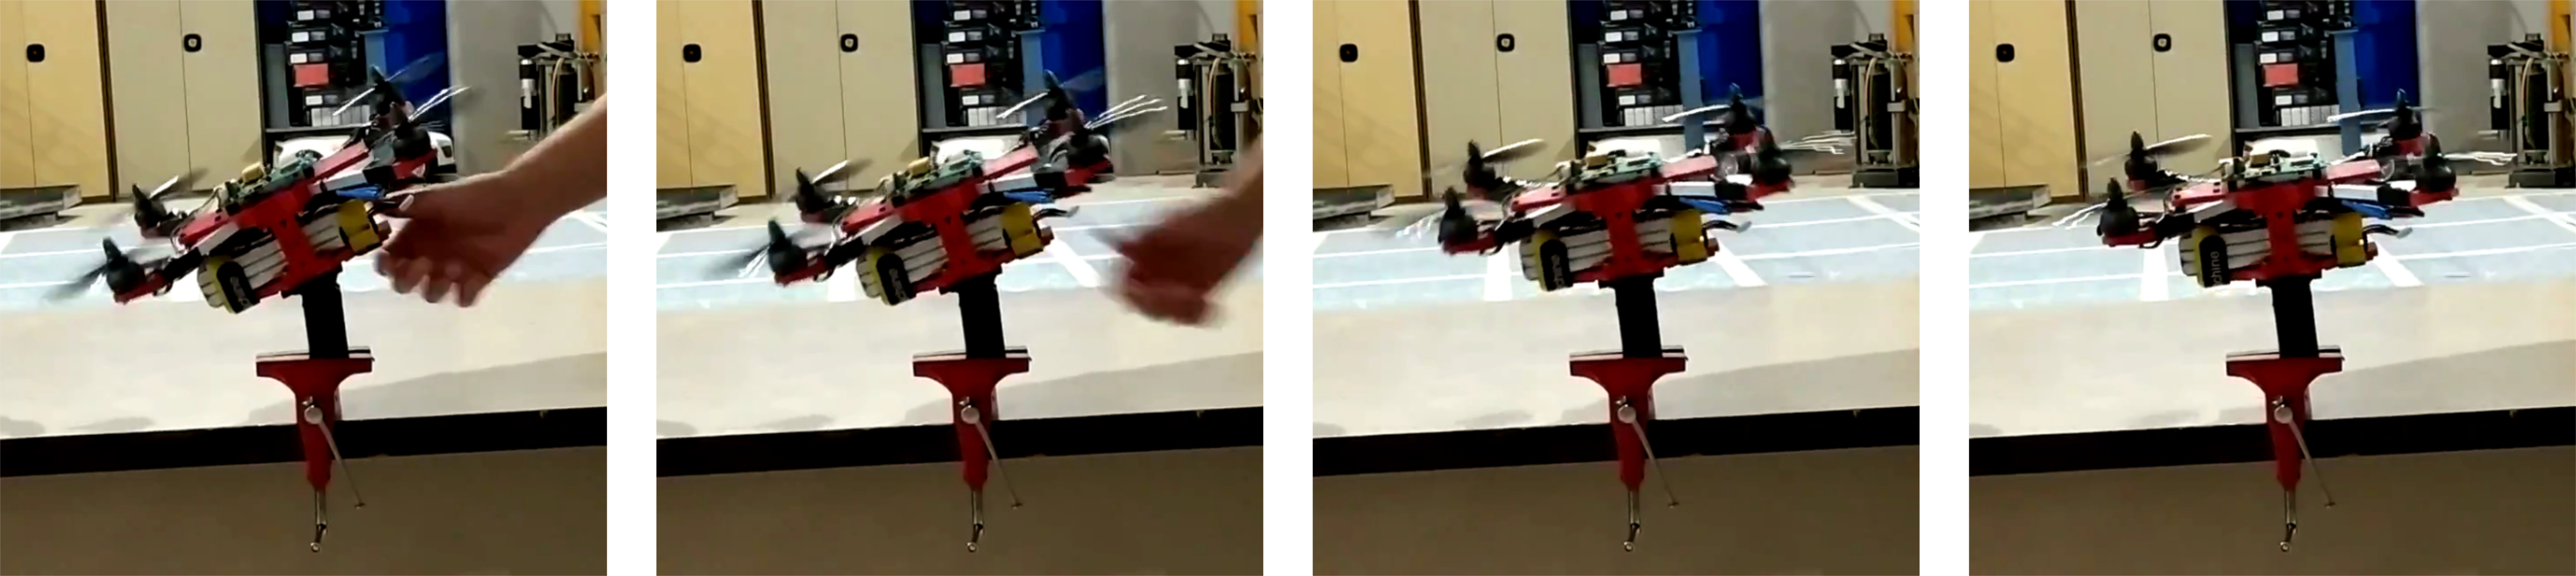
\includegraphics[width=\textwidth]{experimentos/time_lapse_pitch_real}
	\caption{\tb{cambiar}}
	\label{tl_pr}	
\end{figure}

El comportamiento observado es similar al del experimento anterior: el sistema se estabiliza y consigue llegar a la referencia después de perturbarlo de una forma ágil, pero también se observa ruido y un pequeño error de posición en el régimen permanente.

\subsubsection{Control en los 3 Gdl}

En este experimento se ha empleado la rótula de 1 GdL que permite el movimiento en \textit{roll}, \textit{pitch} y \textit{yaw} .
\\

\begin{figure}[htb!]
	\centering
	\includegraphics[width=0.9\textheight,angle=90]{experimentos/3_in_one_matlab}
	\vspace{0.5cm}
	\caption{Estabilización en \textit{roll}, \textit{pitch y \textit{yaw}} simultáneamente}
	\label{tl_pr}	
\end{figure}
\newpage
En este experimento observamos que aumenta el ruido que encontramos en el régimen permanente en \textit{pitch} y en \textit{roll}, aunque se disminuye el error de posición que veíamos en los experimentos anteriores. Por otro lado el controlador de \textit{yaw} es el menos ruidoso, pero también el más lento.
\begin{figure}[htb!]
	\centering
	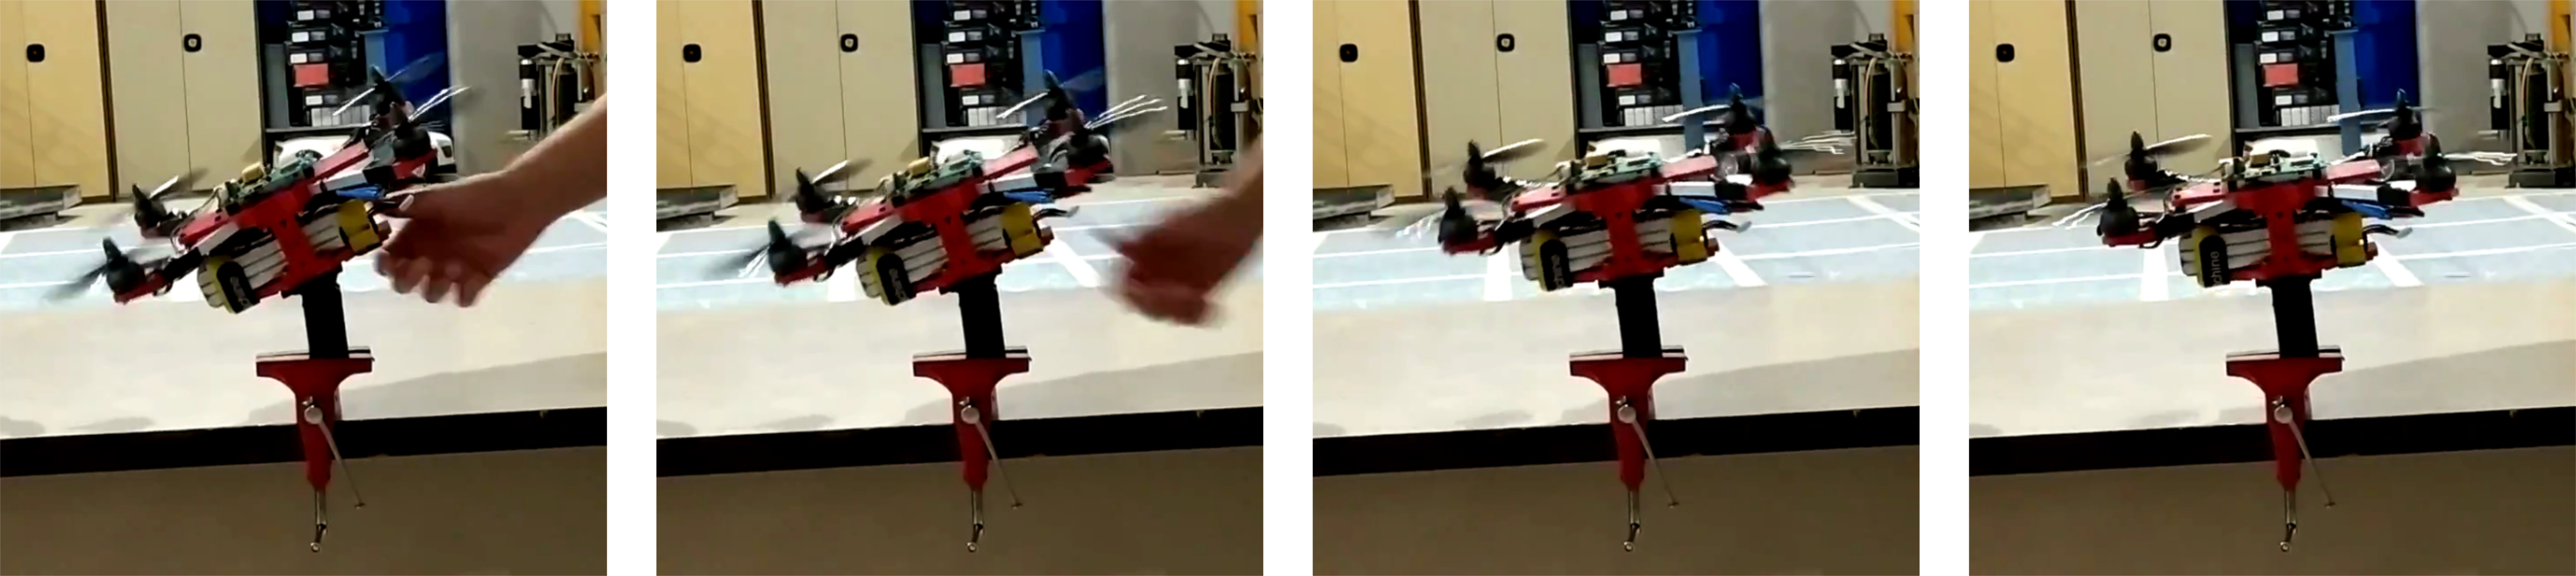
\includegraphics[width=\textwidth]{experimentos/time_lapse_pitch_real}
	\caption{\tb{cambiar}}
	\label{mat_lab_graph}	
\end{figure}



%\begin{figure}[htb!]
%	\centering
%	\begin{tabular}{|c|c|c|c|}
%	\hline
%	&$K_p$&$K_i$&$K_d$\\
%	\hline	
%	$PID_{\dot\varphi}$ &0.003 & 0.0002  & 0.004\\
%	\hline
%	$ PID_{\dot \theta}$ &0.003 & 0.0002  & 0.004\\
%	\hline
%	$ PID_{\dot \psi}$ &0.003 & 0.0002  & 0.004\\
%	\hline
%	\end{tabular}\\
%
%\end{figure}
	\input{discusion/discusion}
	\chapter{Conclusiones y trabajo futuro}

Durante el transcurso de este proyecto se ha conseguido desarrollar una plataforma, que permite estudiar los distintos algoritmos de control, con los que se puede estabilizar a un cuadricóptero. A continuación se hablara sobre las conclusiones que se han extraído durante este proceso y las posibles líneas de mejora que se podrían realizar en un futuro.

\section{Conclusiones}

Los objetivos principales que se plantearon al comienzo del proyecto consistían en: desarrollar un autopiloto propio capaz de ejecutar distintos algoritmos de control para cuadricópteros, desarrollar una plataforma de vuelo para poder probar este autopiloto y los algoritmos de forma segura e investigar sobre la posibilidad de emplear distintos algoritmos de aprendizaje por refuerzo para el control de actitud de la aeronave. A continuación desgranaremos las conclusiones que se han extraído de cada uno de estos objetivos y las posibles mejoras que se pueden realizar de cada uno.

\subsubsection{Autopiloto}
Se ha conseguido desarrollar un autopiloto funcional, capaz de estimar el estado de la aeronave y estabilizarse, cerrando un bucle interno de control y generando los comandos necesarios para controlar los motores. En este autopiloto se ha integrado la etapa de potencia necesaria para que sea posible alimentar al mismo directamente desde la batería, por lo que integra en una única PCB una gran cantidad de funcionalidades que no son habituales en los autopilotos comerciales, como por ejemplo la conexion WiFi, lo que ha permitido recabar los datos en tiempo real de forma sencilla. Sin embargo, las pistas que alimentan los motores a través de placa no se encuentran lo suficientemente ventiladas, por lo que se calientan demasiado.

\subsubsection{Plataforma de vuelo}
La plataforma de vuelo, ha permitido llevar a cabo los experimentos realizados de una forma segura y controlada. Debido a que la inmensa mayoría de las piezas han sido fabricadas mediante técnicas de impresión 3D, ha sido posible realizar variaciones de la plataforma de forma rápida y sencilla. Es por ésto que ,  se han diseñado varios componentes intercambiables, para poder modificar la configuración de los experimentos, lo que ha sido crucial para poder realizar el ajuste los parámetros del PID en las pruebas reales. El inconveniente que tiene la impresión 3D empleando PLA, es la fragilidad de algunas piezas, como por ejemplo, la unión esférica del banco de pruebas.

\subsubsection{Algoritmos basados en aprendizaje por refuerzo}

Uno de los retos que más tiempo han requerido, ha sido conseguir que los algoritmos propuestos, convergieran a una política óptima. Ha sido un proceso iterativo que ha tomado mucho tiempo hasta que se consiguió la convergencia del primer algoritmo. Posteriormente se realizaron muchas modificaciones de los hiperparámetros con el ánimo de mejorar el comportamiento del agente. Finalmente se ha conseguido aplicar varios algoritmos del estado del arte, consiguiendo , en algunos casos como en el del TRPO, buenos rendimientos.


\section{Trabajo futuro}

	
	
	\cfoot{\thepage}
	\pagenumbering{arabic}
	
	\nocite{*}
	\bibliographystyle{IEEEtran}
	\bibliography{IEEEabrv,workBibliography}
\end{document}
